% !TEX TS-program = pdflatex
% !TEX encoding = UTF-8 Unicode

% This is a simple template for a LaTeX document using the "article" class.
% See "book", "report", "letter" for other types of document.

\documentclass[11pt]{article} % use larger type; default would be 10pt

\usepackage[utf8]{inputenc} % set input encoding (not needed with XeLaTeX)

%%% Examples of Article customizations
% These packages are optional, depending whether you want the features they provide.
% See the LaTeX Companion or other references for full information.

%%% PAGE DIMENSIONS
\usepackage{geometry} % to change the page dimensions
\geometry{a4paper} % or letterpaper (US) or a5paper or....
% \geometry{margin=2in} % for example, change the margins to 2 inches all round
% \geometry{landscape} % set up the page for landscape
%   read geometry.pdf for detailed page layout information

\usepackage{graphicx} % support the \includegraphics command and options

% \usepackage[parfill]{parskip} % Activate to begin paragraphs with an empty line rather than an indent

%%% PACKAGES
\usepackage{booktabs} % for much better looking tables
\usepackage{array} % for better arrays (eg matrices) in maths
\usepackage{paralist} % very flexible & customisable lists (eg. enumerate/itemize, etc.)
\usepackage{verbatim} % adds environment for commenting out blocks of text & for better verbatim
\usepackage{subfig} % make it possible to include more than one captioned figure/table in a single float
% These packages are all incorporated in the memoir class to one degree or another...

%%% HEADERS & FOOTERS
\usepackage{fancyhdr} % This should be set AFTER setting up the page geometry
\pagestyle{fancy} % options: empty , plain , fancy
\renewcommand{\headrulewidth}{0pt} % customise the layout...
\lhead{}\chead{}\rhead{}
\lfoot{}\cfoot{\thepage}\rfoot{}

%%% SECTION TITLE APPEARANCE
\usepackage{sectsty}


\allsectionsfont{\sffamily\mdseries\upshape} % (See the fntguide.pdf for font help)
% (This matches ConTeXt defaults)

%%% ToC (table of contents) APPEARANCE
\usepackage[nottoc,notlof,notlot]{tocbibind} % Put the bibliography in the ToC
\usepackage[titles,subfigure]{tocloft} % Alter the style of the Table of Contents
\renewcommand{\cftsecfont}{\rmfamily\mdseries\upshape}
\renewcommand{\cftsecpagefont}{\rmfamily\mdseries\upshape} % No bold!

%%% END Article customizations


\usepackage[bulgarian]{babel}
\usepackage{physics}
\usepackage{amsmath}
\usepackage{centernot}
\usepackage{url}
\usepackage{graphicx}
\graphicspath{ {.} }
\usepackage{amsfonts}
\usepackage{xcolor}
\usepackage{enumitem}
\usepackage{systeme}
\usepackage{listings}
\usepackage[cache=false]{minted}
\usepackage{csquotes}
\setquotestyle{english}



%%% The "real" document content comes below...

\title{22. Използване на XML за структуриране, валидация, обработка и представяне на документно съдържание}
\author{Play4u}
%\date{} % Activate to display a given date or no date (if empty),
         % otherwise the current date is printed
         

\newcommand{\lrangle}[1]{\left\langle #1 \right\rangle}

\newcommand{\oversetModels}[1]{\overset{#1}{\models}}

\newcommand{\italicBold}[1]{\textbf{\emph{#1}}}

\newcommand{\definition}{\italicBold{Дефиниция: }}
\newcommand{\theorem}{\italicBold{Теорема: }}
\newcommand{\lemma}{\italicBold{Лема: }}
\newcommand{\proof}{\italicBold{Доказателство: }}
\newcommand{\statement}{\italicBold{Твърдение: }}
\newcommand{\source}{\italicBold{Източник: }}

\newcommand{\integral}[4]{\displaystyle \int_{#1}^{#2}#3\,#4}

\newcommand{\redText}[1]{\textcolor{red}{#1}}

\newcommand{\curlies}[1]{\{#1\}}
\newcommand{\overbar}[1]{\mkern 1.5mu\overline{\mkern-1.5mu#1\mkern-1.5mu}\mkern 1.5mu}

\newcommand{\xml}[1]{
\begin{minted}{xml}
#1
\end{minted}
}

\newcommand{\enumNum}{\renewcommand{\theenumi}{\arabic{enumi}}}
\newcommand{\enumlet}{\renewcommand{\theenumi}{\alph{enumi}}} 

\begin{document}
\maketitle

\italicBold{Конспект: } Изложението на въпроса трябва да включва следните по-съществени елементи:

\enumNum
\begin{enumerate}[noitemsep]
	\item Добре структуриран XML - основни концепции, XML йерархии
	\item XML валидация чрез Documet Type Definitions(DTD) - цели на валидирането, DTD структура, синтаксис
	\item XML валидация чрез XML схема - спецификация, типове данни, фасети, структури. Сравнение с DTD.
	\item Използване на XSLT (eXtensible StyleSheet Transformations) и XPath за алокиране, манипулиране и представяне на XML съдържание.
	\item Използване на DOM(Document Object Model) и SAX(Simple API for XML) за обработката на XML документи - основни интерфейси на DOM и SAX и начини за използването им. Сравнение между DOM и SAX.\\\par
\end{enumerate}

Extensible Markup Language (XML) is a markup language that defines a set of rules for encoding documents in a format that is both human-readable and machine-readable.
Extensible Markup Language (XML) e markup език, който определя правила за форматиране на документи по начин, който е еднвоременно четим от машини и хора. 

\section{Добре-структуриран XML}
Добре-структурираният XML документ е такъв, който изпълнява синтактичните правила, дефинирани от спецификацията на XML 1.0. Тя твърди, че документа трябва трябва да изпълнява както физическите така и логическите структури дефинирани в спецификацията.\\
На най базово ниво добре-структурираните документи изискват:
\begin{itemize}[noitemsep]
	\item Съдържанието им да е дефинирано
	\item Различното съдържание да е обозначено чрез начален и краен таг
	\item Съдържанието да е добре nest-нато(\textit{insert translation here}) - родителите да са в корена; децата в родителите 
\end{itemize}
За да бъде добре-структуриран документа, някои правила за декларацията и работата с entities трябва да бъдат дефинирани. Таговете са case-sensitive; атрибутите са обозначени от двойни кавички; празните елементи се придържат към всички останали правила; тагове, в различни нива на йерархията които се припокриват правят документа невалиден; в най-добрия случай един добре-структуриан XML документ отговаря на целите на XML като маркъп език. Някои други синтактични правила включват:\\
\begin{itemize}[noitemsep]
	\item Документа трябва да съдържа само легални Unicode символи
	\item Нито един от специалните символи като "<" и "\&" са в документа, освен когато изпълняват техните сепциални markup роли
	\item Началните и крайни тагове на всички елементи са правилно nest-нати и не се припокриват. На всеки един начален таг трябва да отговаря краен таг.
	\item Таговете са case-sensitive. Началните и крайни тагове трябва да са едни и същи. Имената на таговете не трябва да съдържат нито един от символите: 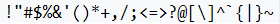
\includegraphics[scale=0.8]{chars.png}, нито "space", нито пък могат да започват със символите \enquote{-}, \enquote{.}, или пък с число.
	\item Има един коренов елемент, който съдържа всички останали елементи.
\end{itemize}

Добре структурираните документи също контрастират разликата между валиден и добре-структуриран XML документ. Според W3C, валидните документи са тези, валидирани спрямо DTD, докато добре-структурираните трябва просто да се придържат към гореспоменатите правила. 
\subsection{XML namespace}
В XML, имената на елементите се дефинират от разработчика. Това означава, че когато смесваме различни XML документи от различни XML апликации могат да настъпят конфликти. Пр.: следният XML носи информация за таблиците в един HTML документ.\\
\begin{minted}{xml}
<table>
  <tr>
    <td>Apples</td>
    <td>Bananas</td>
  </tr>
</table>
\end{minted}

А следният документ описва информация за маса(table).\\
\begin{minted}{xml}
<table>
  <name>African Coffee Table</name>
  <width>80</width>
  <length>120</length>
</table>
\end{minted}
Ако използваме и двата XML документа, ще настъпи конфликт, тъй като и двата съдържат <table> елемент.\\
Решението е да използваме XML namespaces. Те представляват префикс в XML, с дефиниран за префикса namespace - обикновено някакъв URI, който определя "домейна" на използвания таг. Декларацията на namespace има следния синтаксис: xmlns:prefix=\enquote{URI}. Така за да решим проблема, може да имаме следния XML:\\
\begin{minted}{xml}
<root>
<h:table xmlns:h="http://www.w3.org/TR/html4/">
  <h:tr>
    <h:td>Apples</h:td>
    <h:td>Bananas</h:td>
  </h:tr>
</h:table>

<f:table xmlns:f="https://www.w3schools.com/furniture">
  <f:name>African Coffee Table</f:name>
  <f:width>80</f:width>
  <f:length>120</f:length>
</f:table>
</root>
\end{minted}
Съшо така можем да използваме и т.нар. namespace по подразбиране - за да не се налага да поставяме префикси във всички деца на дадения елемент. Така горния пример ще стане:\\
\begin{minted}{xml}
<root>
<table xmlns="http://www.w3.org/TR/html4/">
  <tr>
    <td>Apples</td>
    <td>Bananas</td>
  </tr>
</table>

<table xmlns="https://www.w3schools.com/furniture">
  <name>African Coffee Table</name>
  <width>80</width>
  <length>120</length>
</table>
</root>
\end{minted}

\section{DTD}
DTD - Document Type Definition е XML документ, който дефинира структурата и позволените елемти и атрибути в друг XML документ . Чрез DTD, различни организации могат да се споразумеят на един общ стандарт, който да използват при размяната на данни помежду си чрез XML. Също така едно приложение може да използва DTD да валидира валидността на данните в даден XML документ. Можем да дефинираме DTD както в самия XML който, искаме да валидираме, така и извън него, в отделен файл. Пример за Вътрешна декларация на DTD:
\begin{minted}{xml}
<?xml version="1.0"?>
<!DOCTYPE note [
<!ELEMENT note (to,from,heading,body)>
<!ELEMENT to (#PCDATA)>
<!ELEMENT from (#PCDATA)>
<!ELEMENT heading (#PCDATA)>
<!ELEMENT body (#PCDATA)>
]>
<note>
<to>Tove</to>
<from>Jani</from>
<heading>Reminder</heading>
<body>Don't forget me this weekend</body>
</note>
\end{minted}

Този DTD се интепретира по следния начин:
\begin{itemize}[noitemsep]
	\item \textbf{!DOCTYPE note} дефинира, че кореновият елемент на този документ е \textbf{note}
	\item \textbf{!ELEMENT to} дефинира, че елементът \textbf{to} трябва да е от тип \enquote{\#PCDATA}
	\item \textbf{!ELEMENT from} дефинира, че елементът \textbf{from} трябва да е от тип \enquote{\#PCDATA}
	\item \textbf{!ELEMENT heading} дефинира, че елементът \textbf{heading} трябва да е от тип \enquote{\#PCDATA}
	\item \textbf{!ELEMENT body} дефинира, че елементът \textbf{body} трябва да е от тип \enquote{\#PCDATA}
\end{itemize}
 
 А сега ще покажем външна декларация на DTD. Първо, така изглежда документа, който ще валидираме спрямо DTD. Да забележим, че той има референция към външния DTD файл \textbf{note.dtd}.\\
\begin{minted}{xml}
<?xml version="1.0"?>
<!DOCTYPE note SYSTEM "note.dtd">
<note>
  <to>Tove</to>
  <from>Jani</from>
  <heading>Reminder</heading>
  <body>Don't forget me this weekend!</body>
</note>
\end{minted}

Ето го и файла \textbf{\enquote{note.dtd}}, който съдържа DTD-то.
\begin{minted}{dtd}
<!ELEMENT note (to,from,heading,body)>
<!ELEMENT to (#PCDATA)>
<!ELEMENT from (#PCDATA)>
<!ELEMENT heading (#PCDATA)>
<!ELEMENT body (#PCDATA)>
\end{minted}

От гледната точка на DTD, всички XML документи са изградени от следните елементи:
\begin{itemize}[noitemsep]
	\item Елементи
	\item Атрибути
	\item Entities
	\item PCDATA
	\item CDATA
\end{itemize}

\subsection{Елементи}
Основните изграждащи блокове на XML. Те съдържат информацията в документа. Пр.: 
\begin{minted}{xml}
<body>some text</body>
\end{minted}

\subsection{Атрибути}
Атрибутите описват допълнителна информация за атрибутите
\begin{minted}{xml}
<img src="computer.gif" />
\end{minted}

\subsection{Entities}
Тъй като, някой символи има специално значение в XML, като знака за по малко \enquote{<}, който дефинира началото на XML таг.\\
За целта тези елементи се представят чрез референции - за знака \enquote{<}, това е референцията \textbf{\&lt;}. Ето някои от най-използваните референции:\\
\begin{center}
	\includegraphics[scale=0.75]{references.png}
\end{center}

\subsection{PCDATA}
PCDATA е съкращение на Parsed Character Data. Това е текста между отваряюия и затварящия таг в един XML елемент. \textbf{PCDATA e текст, който ще бъде парснат от XML парсъра, т.е. текста ще бъде изследвам за референции и markup.}

\subsection{CDATA}
Обратно, CDATA е текст, който няма да бъде парснат от парсъра.

\subsection{Синтаксис}
Сега ще покажем, само основният синтаксис на DTD. За повече информация, посетете W3C schools.\\
\textit{\textbf{Деклариране на елементи:}}\\
\begin{minted}{dtd}
<!ELEMENT element-name category>
or
<!ELEMENT element-name (element-content)>
\end{minted}

\textit{\textbf{Деклариране на атрибути:}}\\
\begin{minted}{dtd}
<!ATTLIST element-name attribute-name attribute-type attribute-value>
\end{minted}

\textit{\textbf{Деклариране на entitites:}}\\
\begin{minted}{dtd}
<!ENTITY entity-name "entity-value">
\end{minted}
т.е.
\begin{minted}{dtd}
<!ENTITY writer "Donald Duck.">
<!ENTITY copyright "Copyright W3Schools.">
\end{minted}
в XML
\begin{minted}{xml}
<author>&writer;&copyright;</author>
\end{minted}

\section{XML Schema}
XML схемата опсива структурата на един XML документ. Езикът на XML Scema се нарича XML Schema Definition(XSD). Целта на XML Scema е да дефинира позволените изграждащи блокове на един XML документ:
\begin{itemize}[noitemsep]
	\item Елементите и атрибутите които могат да бъдат в един документ
	\item Броя (и реда на) елемнтите-деца
	\item Типовете данни на елементите и атрибутите
	\item Стойности по подразбиране и константни стойности на елементите и атрибутите
\end{itemize}

В екосистемата на XML се използват стотици стандартизирани XML формата. Много от тях са базирани на XML схеми. XML схемата е базирана на XML(и по-силна) алтернатива на DTD.  

\subsection{Основни характеристики на XML Schema}
Типизация на данните - една от най-големите сили на XML схемите.
\begin{itemize}
	\item По-лесно е да описваме позволеното съдържание на документа
	\item По-лесно е да валидираме правилността на данните
	\item По-лесно е да дефинираме фасети (рестрикции) върху данните
	\item По-лесно е да дефинираме data patterns(формати на данните)
	\item По-лесно е да конвертираме данните между различните типове данни 
\end{itemize}

Друга силна характеристика на XML схемите е, че са написани в XML. Това означава, че можем да използваме всички положителни черти на XML в XML схема - XML parsers, editors, XML DOM, XSLT и т.н.

Една основна причина за появата на XML схеми(по подобие на DTD) е, че в пракиката, не е достатъчно един XML да е просто добре структуриран. Това е така, тъй като дори един документ да е добре структуриран, той все още може да съдържа логически грешки.

\subsection{Синтаксис}
Елементът <schema> е кореновият елемент на всяка една XML схема.
\begin{minted}{xml}
<xs:schema>
...
...
</xs:schema>
\end{minted}

Той може да съдържа някои атрибути:
\begin{minted}{xml}
<xs:schema xmlns:xs="http://www.w3.org/2001/XMLSchema"
targetNamespace="https://www.w3schools.com"
xmlns="https://www.w3schools.com"
elementFormDefault="qualified">
\end{minted}

Частта:\\
xmlns:xs="http://www.w3.org/2001/XMLSchema"\\
показва, че елементите и типовете данни, използвани в схемата идват от namespace-a \textbf{http://www.w3.org/2001/XMLSchema}. Също така специфицира, че елементите и типовете данни, които идват от този namespace трябва да бъдат префикснати с \textbf{xs:}.\\\par

Подобно на DTD, XML схемата може да бъде както вътрешна за даден XML документ, така и отделен, външен файл, който се реферира от документа.\\\par

\textit{\textbf{Прост елемент: }} Простият елемент е тип XML елемент, който може да съдържа само текст - не може да съдържа други елемнти или атрибути. Но трябва да поясним, че под просто текст се има предвид всеки един тип данни, дефиниран от XML схема, или дори всеки един тип данни, дефинирани от разработчика. Също така можем да дефинираме и фасети върху \enquote{текста} за да можем да изискване от данните да се конформират по определен стандарт(pattern). Синтаксиса за декларация на прост елемент е:\\
\begin{minted}{xml}
<xs:element name="xxx" type="yyy"/>
\end{minted}
XML схема има много вградени типове данни. Част от най-използваните са:
\begin{itemize}[noitemsep]
	\item xs:string
	\item xs:decimal
	\item xs:integer
	\item xs:boolean
	\item xs:date
	\item xs:time
\end{itemize}

Пример за използването им: Нека имаме XML-a\\
\begin{minted}{xml}
<lastname>Refsnes</lastname>
<age>36</age>
<dateborn>1970-03-27</dateborn>
\end{minted}

тогава следната схема отговаря на него:
\begin{minted}{xml}
<xs:element name="lastname" type="xs:string"/>
<xs:element name="age" type="xs:integer"/>
<xs:element name="dateborn" type="xs:date"/>
\end{minted}

Простите елементи могат да имат стойност по подразбиране ИЛИ константна стойност.\\
Стойността по подразбиране автоматично се присвоява на елемента, когато друга такава не е налична. В следващия пример стойността по подразбиране е \enquote{red}.
\begin{minted}{xml}
<xs:element name="color" type="xs:string" default="red"/>
\end{minted}

Константната стойност също автоматично се присовява елемента, но не може да й се присвоява друга стойност. 
\begin{minted}{xml}
<xs:element name="color" type="xs:string" fixed="red"/>
\end{minted}

\textit{\textbf{Атрбитути: }}Съшите правила важат и за атрибутите. Синтаксиса за деклариране на атрибут е:
\begin{minted}{xml}
<xs:attribute name="xxx" type="yyy"/>
\end{minted}

Атрибутите не са задължителни по подразбиране. За да обозначим атрибут като задължителен, трябва да изпозване атрибута \enquote{use} по следния начин: 

\begin{minted}{xml}
<xs:attribute name="lang" type="xs:string" use="required"/>
\end{minted}

Когато даден XML атрибут има дефиниран тип данни, това поставя определени рестрикции върху съдържанието на елемента.  Ако XML елемент е от тип \textbf{xs:date} и съдържа низ като \textbf{Hello world}, то документът няма да бъде валидиран. Чрез XML схема можем да деклраираме собстени рестрикции върху данните, наречени фасети. \\
\textbf{\textit{Фасети: }} Следния пример дефинира елемент \enquote{age} с рестрикция, че стойността на \enquote{age} не може да е по-малка от 0 или по-голяма от 100.
\begin{minted}{xml}
<xs:element name="age">
  <xs:simpleType>
    <xs:restriction base="xs:integer">
      <xs:minInclusive value="0"/>
      <xs:maxInclusive value="120"/>
    </xs:restriction>
  </xs:simpleType>
</xs:element>
\end{minted}
Можем да дефинираме множество различни фасети, използвайки този pattern. За информация за всички възможни фасети, посетете W3C schools.\\\par

\textit{\textbf{Комплексни елементи: }} Това са елементи, които съдържат други елементи и/или атрибути. Има 4 типа комплексни елементи:\\
\begin{itemize}[noitemsep]
	\item празни елементи
	\item елементи, които съдържат само други елементи
	\item елементи, които съдържат само текст
	\item елементи, които съдържат други елементи и текст 
\end{itemize}
Всеки един от тези елементи също така могат да съдържат атрибути. Синтаксиса за дефиниране на комплексен елемент може да се обобщи със следния пример. Нека имаме XML файла:
\begin{minted}{xml}
<employee>
  <firstname>John</firstname>
  <lastname>Smith</lastname>
</employee>
\end{minted}
Една XMl схема, която отговаря на него е следната:
\begin{minted}{xml}
<xs:element name="employee">
  <xs:complexType>
    <xs:sequence>
      <xs:element name="firstname" type="xs:string"/>
      <xs:element name="lastname" type="xs:string"/>
    </xs:sequence>
  </xs:complexType>
</xs:element>
\end{minted}
Тъй като елементите \textbf{firstname} и \textbf{lastname} са дефинирани в елемента \textbf{sequence}, те трябва да са в същия ред в съотвестващия XML документ. В обратния случай, бихме използвали елемента \textbf{choice}.

\subsection{Сравнение с DTD}
Основните предимтва на XML schema пред DTD са следните:
\begin{itemize}[noitemsep]
	\item XML schema поддържа типове
	\item XML schema поддържа рестрикции върху това колко пъти да се съдържа даден елемент
	\item XML schema поддържа енумерации
	\item XML schema се пише на XML, а DTD - не
\end{itemize}

\section{XSLT}
XSL(eXtensible Stylesheet Language) е език за дефиниране на стилове на XML документи.\\
XSLT е съратено от XSL Transformations. Можем да използваме XSLT да трансформираме XML докумети в други XML документи, или други формати като цяло - пр. HTML.\\\par
XSL по подобие, на CSS (като stylesheet езици) - към HTML, се използва за специфициране на това как XML елементите трябва да се изобразяват. XSL не е просто stylesheet език, а се състои от 4 други части:\\
\begin{itemize}[noitemsep]
	\item \textbf{XSLT} - език за трансформиране на XML документи
	\item XPath - език за навигация в XML документи
	\item XSL-FO - език за форматиране на XML документи(не е поддържан от 2013-та година)
	\item XQuery - език за правене на заявки към XML документи \\
\end{itemize}

Чрез XSLT можем да добавяме/премахваме елементи и атрибути в/от изходящия от трансформацията файл. Можем също така да пренареждаме и соритраме елементи, да правим тестове и да вземаме решения на базата да на техните резултати, които да дефинират кои елемти да скриваме, показваме и др. \\
XSLT използва XPath за да навигира сред елементите и атрибутите в XML документи. По време на процеса по трансформация, XSLT използва XPath да дефинира части от документа-източник които трябва да съвпадат с предефинирани от разработчика шаблони.\\\par
XSLT използва елементи от namespace-a \textbf{xmlns:xsl="http://www.w3.org/1999/XSL/Transform} за да свързва шаблона от XSLT файла към действителни стойности от един XML документ.\\
Всеки един XSLT документ има коренов елемент със следния синтаксис:\\
\begin{minted}{xml}
<?xml version="1.0" encoding="UTF-8"?>
<xsl:stylesheet version="1.0"
xmlns:xsl="http://www.w3.org/1999/XSL/Transform">
\end{minted}
Сега ще опишем някои от по-важните XSLT елементи.

\subsection{xsl:value-of}
Елементът <xsl:value-of> може да се използва за извличане на стойност от XML елемент и добавянето й към изходния поток на трансформацията. Той има следния синтаксис:
\begin{minted}{xml}
<xsl:value-of select="expression" disable-output-escaping="yes|no" />
\end{minted}
Атрибутът \enquote{select} е задължителен и трябва да има стойност XPath израз, който специфицира от кой елемент/атрибут да се извлече търсената стойност. \enquote{disable-output-escaping} - опционален атрибут, който показва, дали специални символи като (<) трябва да се трансформират в изходния поток така както се срещат във входния поток. Стойността по подразбиране е \enquote{no}.

\subsection{xsl:for-each}
Елементът <xsl:for-each> итерира през всеки един елемент в множеството от елементи, дефинирано от атрибута му \enquote{select}. Има синтаксис от вида:
\begin{minted}{xml}
<xsl:for-each select="expression">
  <!-- Content -->
</xsl:for-each>
\end{minted}
\enquote{select} е XPath израз.

\subsection{xsl:apply-templates}
Елементът <xsl:apply-templates> прилага шаблонно правило към текущия елемент или към неговите деца. Има синтаксис:
\begin{minted}{xml}
<xsl:apply-templates select="expression" mode="name">
  <!-- Content:(xsl:sort|xsl:with-param)* -->
</xsl:apply-templates>
\end{minted}

Разбира се има още много XSLT елементи, които могат да се използват по множество различни начини за алокиране, манипулиране и проекция на данни. За повече информация посетете W3C schools.

\subsection{XPath}
Няколко пъти вече споменаваме, че някои XSLT елементи имат атрибути, които имат стойност от тип XPath израз. Нека сега да обясним как да използваме XPath. \\
\\ Връх = елемент или атрибут
XPath използва path изрази, за да избира множество върхове в един XML документ. Върховете се избират, следвайки пътя или т.нар. стъпки. Най-полезните Path изрази са изброени отдолу.\\
\begin{center}
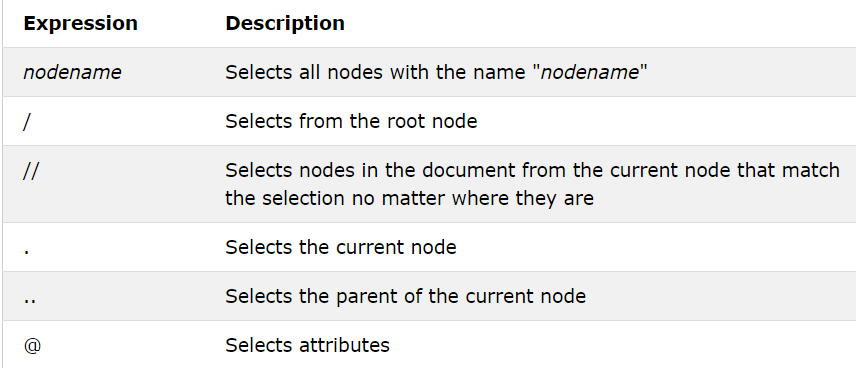
\includegraphics[scale=0.75]{PathExpressions.png}
\end{center}

В слеващата таблица ще опишем няколко path израза и резултатът от тяхното изпълнение.
\begin{center}
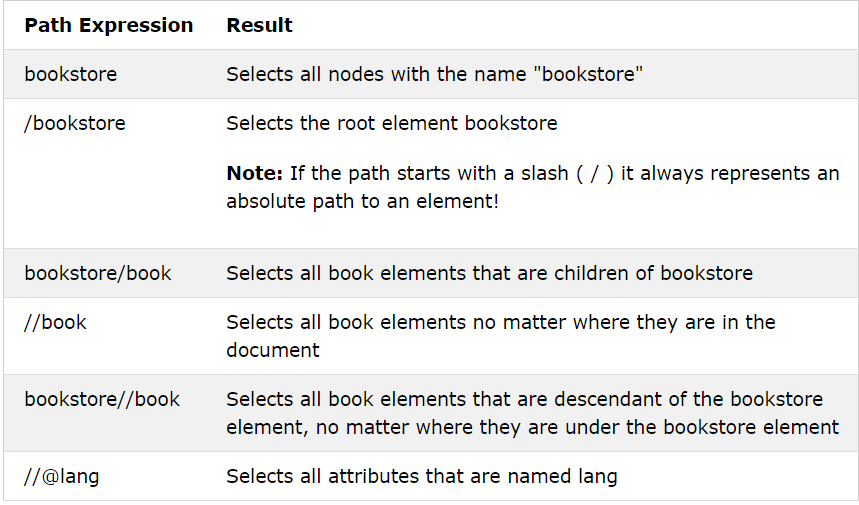
\includegraphics[scale=0.75]{PathExpressionResults.png}
\end{center}

Предикати: предикатите се използват за да намират определен връх или връх който съдържа определена стойност. Предикатите винаги са оградени от квадратни скоби([]). В таблицата по-долу ще опишем някои от най-използваните предикати, както и резултатите от тяхното изпълнение. 

\begin{center}
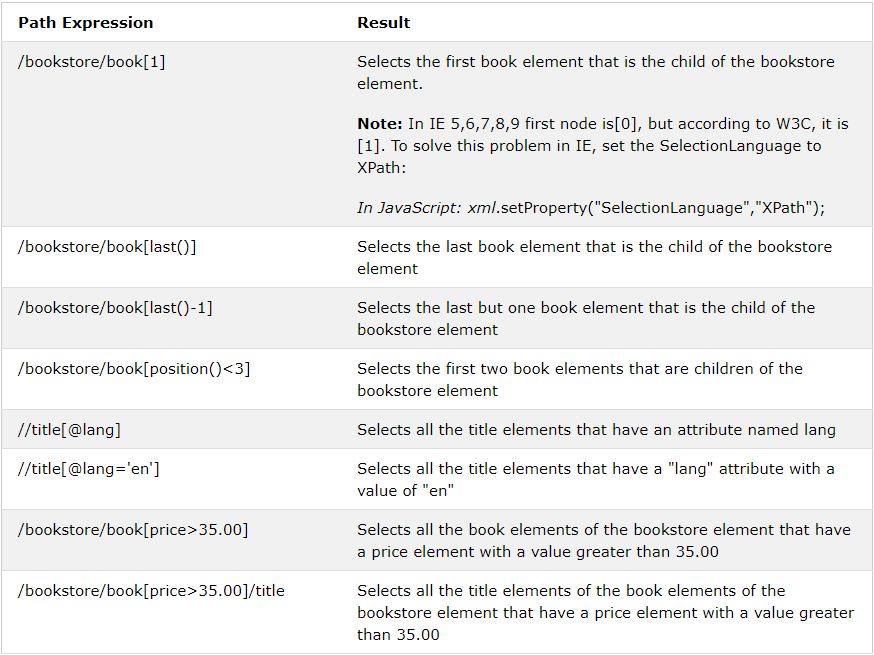
\includegraphics[scale=0.75]{Predicates.png}
\end{center}

Има и други XPath изрази. За повече информация - W3C schools.

\section{DOM и SAX}
\subsection{DOM}
DOM (Document Object Model) дефинира стандарт за достъп до документи и тяхната манипулация. \\
XML DOM-ът дефинира стандартен начин за достъп и манипулация на XML документи. Той предоставя XML документът като дървовидна структура. \\\par
DOM-ът представя XML като множество от върхове. Тези върхове могат да бъдат достъпвани чрез JavaScript или други програмни езици. Ние ще използваме JavaScript за да покажем функционалността на DOM-a. Програмният интерфейс на DOM-a се дефинира от множество стандартни свойства(properties) и методи. \\
\textbf{Свойствата} обикновено са нещо което \textbf{е} - пр.  името на върха \textbf{е} \enquote{book}\\
\textbf{Методите} обикновено са нещо което \textbf{се върши} - пр. delete \enquote{book}\\\par

\textbf{XML DOM свойства.} Ето няколко типични DOM свойства:
\begin{itemize}[noitemsep]
	\item x.nodeName - името на x
	\item x.nodeValue - стойността на x
	\item x.parentNode - родителският връх на x
	\item x.childNodes - върховете-деца на x
	\item x.attributes - върховете-атрибути на x\\
\end{itemize}
В гореописаните, x е обект от тип node(връх).\\\par

\textbf{XML DOM методи.}
\begin{itemize}[noitemsep]
	\item x.getElementsByTagName(name) - връща всички елементи със специфицираното име на таг
	\item x.appendChild(node) - вкарва върха node в x
	\item x.removeChild(node) - премахва детето node от x\\
\end{itemize}
В гореописаните, x е обект от тип node(връх).\\\par

Ще демонстрираме използването на DOM-a със следния пример.: Нека имаме следния XML документ:
\begin{minted}{xml}
<?xml version="1.0" encoding="UTF-8"?>
<bookstore>

  <book category="cooking">
    <title lang="en">Everyday Italian</title>
    <author>Giada De Laurentiis</author>
    <year>2005</year>
    <price>30.00</price>
  </book>

  <book category="children">
    <title lang="en">Harry Potter</title>
    <author>J K. Rowling</author>
    <year>2005</year>
    <price>29.99</price>
  </book>

</bookstore>
\end{minted}
Следният код взема текстовата стойност на пръвия елемент от тип <title> и я присвоява на променливата \textbf{txt}.
\begin{minted}{javascript}
txt = xmlDoc.getElementsByTagName("title")[0].childNodes[0].nodeValue;
\end{minted}

\subsection{SAX}
SAX(Simple API for XML) е базиран на събития, онлайн алгоритъм за парсване на XML документи. SAX предоставя алтернатива за четене на данни от XML, различна от предоставената такава от DOM. За разлика от DOM, който изгражда пълното абстрактно синтактично дърво на XML документа, SAX парсърите работят върху всяко една част от XML документа в последователност, \enquote{изстрелвайки(firing)} събития, преминавайик през различните XML елементи. Това се случва с едно единствено преминаване през входящия поток(документа).\\\par

\textit{\textbf{Плюсове: }}A SAX parser only needs to report each parsing event as it happens, and normally discards almost all of that information once reported (it does, however, keep some things, for example a list of all elements that have not been closed yet, in order to catch later errors such as end-tags in the wrong order). Thus, the minimum memory required for a SAX parser is proportional to the maximum depth of the XML file (i.e., of the XML tree) and the maximum data involved in a single XML event (such as the name and attributes of a single start-tag, or the content of a processing instruction, etc.).

This much memory is usually considered negligible. A DOM parser, in contrast, has to build a tree representation of the entire document in memory to begin with, thus using memory that increases with the entire document length. This takes considerable time and space for large documents (memory allocation and data-structure construction take time). The compensating advantage, of course, is that once loaded any part of the document can be accessed in any order.

Because of the event-driven nature of SAX, processing documents is generally far faster than DOM-style parsers, so long as the processing can be done in a start-to-end pass. Many tasks, such as indexing, conversion to other formats, very simple formatting and the like can be done that way. Other tasks, such as sorting, rearranging sections, getting from a link to its target, looking up information on one element to help process a later one and the like require accessing the document structure in complex orders and will be much faster with DOM than with multiple SAX passes.\\\par

\textit{\textbf{Минуси: }}The event-driven model of SAX is useful for XML parsing, but it does have certain drawbacks.

Virtually any kind of XML validation requires access to the document in full. The most trivial example is that an attribute declared in the DTD to be of type IDREF, requires that there be only one element in the document that uses the same value for an ID attribute. To validate this in a SAX parser, one must keep track of all ID attributes (any one of them might end up being referenced by an IDREF attribute at the very end); as well as every IDREF attribute until it is resolved. Similarly, to validate that each element has an acceptable sequence of child elements, information about what child elements have been seen for each parent must be kept until the parent closes.

Additionally, some kinds of XML processing simply require having access to the entire document. XSLT and XPath, for example, need to be able to access any node at any time in the parsed XML tree. Editors and browsers likewise need to be able to display, modify, and perhaps re-validate at any time. While a SAX parser may well be used to construct such a tree initially, SAX provides no help for such processing as a whole.


\end{document}






